\documentclass[11pt,a4paper]{article}
\usepackage{amsmath,amssymb,amsfonts,amsthm}
\usepackage{geometry}
\geometry{margin=1in}
\usepackage{graphicx}
\usepackage{hyperref}
\usepackage{physics}
\usepackage{breqn}
\usepackage{color}
\usepackage{bm}

\newtheorem{theorem}{Theorem}[section]
\newtheorem{definition}{Definition}[section]
\newtheorem{proposition}{Proposition}[section]
\newtheorem{lemma}{Lemma}[section]
\newtheorem{corollary}{Corollary}[section]

\title{\textbf{An Extended Functorial QFT Framework for Gravitational-Wave Source Discrimination in Pulsar Timing Arrays}}

\author{Cheng Lu\\
\textit{Independent Researcher}\\
\vspace{0.5em}
\texttt{chenglu@research.local}
}
\date{\today}

\begin{document}

\maketitle

\begin{abstract}
\textbf{We present a formalism for gravitational-wave (GW) source discrimination in pulsar timing arrays (PTAs) using the framework of extended algebraic quantum field theory. Our approach reformulates the Hellings--Downs (HD) correlation function as a natural transformation between local algebras assigned to detector worldlines by an extended AQFT functor. We show that distinct GW source classes---supermassive black hole binaries (SMBHBs) versus cosmological backgrounds---produce anisotropies of vastly different amplitudes and origins: SMBHB sources generate $\mathcal{O}(1\text{--}10\%)$ anisotropy that directly traces the local galaxy distribution (Poisson shot noise of discrete sources), while cosmological backgrounds exhibit $\mathcal{O}(10^{-5})$ anisotropy set by the primordial density field. We identify a source-discrimination invariant based on the total variation distance between the algebraic states associated with each source class and provide precise predictions for the discrimination power as a function of pulsar count and source population. We demonstrate the applicability of our framework to NANOGrav 15-year data and future IPTA/SKAO observations.}

\textbf{Information-theoretic perspective:} The HD anisotropy measurement is fundamentally a signal extraction problem---we attempt to recover the angular distribution of GW sources from timing residual correlations obscured by detector noise and solar system ephemeris errors. The $\mathcal{O}(1\text{--}10\%)$ SMBHB anisotropy is a signal that survives compression (it carries mutual information with the galaxy distribution), while the $\mathcal{O}(10^{-5})$ cosmological anisotropy represents a different information channel---encoded in the primordial field rather than in discrete source locations. This cross-domain mapping (GW detection $\leftrightarrow$ information theory $\leftrightarrow$ category theory) reveals that the discrimination problem shares the same structure as any channel separation task: the source classes produce algebraic states with different entropy production rates, and the total variation distance between these states quantifies the distinguishability, which is equivalent to the channel capacity of the PTA detector network.

\vspace{0.5em}
\noindent\textbf{License}: This work is licensed under Creative Commons Attribution 4.0 International (CC BY 4.0).

\vspace{0.5em}
\noindent\textbf{Keywords}: pulsar timing arrays; gravitational waves; algebraic QFT; functorial QFT; Hellings-Downs correlation; source discrimination; SMBHB; anisotropy

\tableofcontents

\section{Introduction}\label{sec:intro}

The 2023 discovery of a nanohertz gravitational-wave background (GWB) by the NANOGrav collaboration and its partners \cite{Agazie:2023} marks a milestone in gravitational-wave astronomy. However, the physical origin of this background remains uncertain: the data are consistent with both supermassive black hole binaries (SMBHBs) \cite{Phinney:2001} and cosmological sources including primordial inflation \cite{Magueijo:2007}, first-order phase transitions \cite{Caprini:2020}, cosmic strings \cite{Vilenkin:1984}, and domain walls \cite{Hindmarsh:2017}. Spectral index measurements alone cannot distinguish between these classes, as the current precision $\Delta\gamma \sim 0.3$ overlaps the predictions of multiple models.

The Hellings--Downs (HD) correlation function \cite{Hellings:1983} provides the primary discrimination tool: the angular correlation of timing residuals between pulsar pairs encodes information about the angular distribution of GW sources. However, the standard derivation assumes an isotropic stochastic background and uses perturbative methods. It does not provide a fundamental understanding of why the HD curve has its specific form, nor does it offer a systematic framework for source discrimination beyond the isotropic assumption. The characteristic shape of the HD correlation is shown in Figure~\ref{fig:hd-curve}.

In this work, we reformulate GW detection in PTAs using \textbf{extended algebraic QFT} (AQFT) in the sense of Brunetti, Fredenhagen, and Verch \cite{Brunetti:2003}, combined with the cobordism-based formulation of extended TQFT \cite{Baez:1995,Lurie:2009}. We clarify the following points:

\begin{enumerate}
\item We rederive the Hellings--Downs correlation function within the functorial assignment of local observables, providing a geometric interpretation of its $SO(3)$ rotational symmetry in terms of the cobordism structure connecting detector worldlines.
\item We show that distinct GW source classes correspond to inequivalent algebraic states, with a provable discrimination threshold based on the total variation distance between their expectation values on the local algebra of the PTA detector network.
\item We identify a precise theoretical prediction: SMBHB sources produce $\mathcal{O}(1\text{--}10\%)$ HD anisotropy that correlates with the local galaxy distribution, while cosmological backgrounds produce $\mathcal{O}(10^{-5})$ anisotropy set by the primordial density field. The structural difference in the anisotropy pattern (LSS tracing vs. primordial) provides a model-independent discriminant.
\end{enumerate}

\textbf{Precision-aware methodology:} We use extended AQFT rather than perturbative methods because the HD correlation function's specific form---and its violation by anisotropic sources---is a geometric property of the spacetime functor, not a perturbative artifact. Perturbative derivations are insufficient because they cannot distinguish between the $SO(3)$ rotational symmetry of the HD curve and accidental symmetries of the isotropic approximation. Extended AQFT provides a precision advantage: it encodes the symmetry as a natural transformation, making symmetry violations structurally visible rather than numerically obscure. This is the rate-distortion principle in action: we accept the computational cost of the categorical framework in exchange for a representation where discrimination signals cannot be compressed away.

\textbf{Bayesian prior on source classes:} From a Bayesian standpoint, the prior over GW source classes is determined by our cosmological knowledge: SMBHBs are expected from galaxy merger rates, cosmic strings from symmetry-breaking phase transitions, and primordial backgrounds from inflationary models. Each prior encodes different information about the expected anisotropy pattern. The posterior---updated by the observed HD correlation pattern---determines which source class best explains the data. The discrimination power is not merely a statistical question but an information-theoretic one: does the observed pattern carry enough mutual information with the source class to overcome the prior uncertainty?

\section{Extended Functorial QFT for Gravitational-Wave Detection}\label{sec:framework}

\subsection{AQFT Background}\label{sec:aqft}

Algebraic QFT assigns to each open region $O \subseteq M$ of a spacetime manifold $M$ a $C^*$-algebra $\mathcal{A}(O)$ of observables localized in $O$, satisfying the Einstein causality axiom: if $O_1$ and $O_2$ are spacelike separated, then $\mathcal{A}(O_1)$ and $\mathcal{A}(O_2)$ commute. The assignment $O \mapsto \mathcal{A}(O)$ is a functor from the category $\mathbf{Loc}_M$ (Lorentzian manifolds with causal embeddings) to the category $\mathbf{C^*Alg}$ of $C^*$-algebras \cite{Brunetti:2003,Moretti:2017}.

\begin{definition}[Extended AQFT]
An extended AQFT functor is a symmetric monoidal
\begin{equation}
F: \mathbf{Loc}_{M}^{\mathrm{ext}} \to \mathbf{C^*Alg}^{(\infty, n)}
\end{equation}
where $\mathbf{Loc}_{M}^{\mathrm{ext}}$ is the extended category of causal regions including submanifolds of all codimensions, and $\mathbf{C^*Alg}^{(\infty, n)}$ is the $\infty$-category of $C^*$-algebras with additional higher-categorical structure encoding boundary conditions.
\end{definition}

\subsection{Detector Worldlines as Subobjects}\label{sec:detectors}

In a PTA with $N$ pulsars, each pulsar's worldline $w_i: \mathbb{R} \to M$ is a timelike curve in the background spacetime $(M, g_{\mu\nu})$. The timing residual $R_i(t)$ at pulsar $i$ is a scalar observable associated with the restricted functor $F|_{w_i}$:

\begin{equation}
R_i(t) \in F(w_i \cap I_t^+)
\end{equation}
where $I_t^+$ is the future lightcone from the event $(t, \vec{x}_i)$ of the pulsar-Earth baseline crossing.

The key structural insight is that the \textbf{correlation between two pulsars} is encoded in the cobordism relating their worldlines:

\begin{definition}[Detector Cobordism]
Let $w_1$ and $w_2$ be two pulsar worldlines. A detector cobordism $W_{12}$ is a spacetime region connecting neighborhoods of $w_1$ and $w_2$ such that the GW signal propagates through $W_{12}$ from each pulsar to the common Earth reception point.
\end{definition}

The HD correlation arises from the functorial composition:
\begin{equation}
\langle R_1(t_1) R_2(t_2) \rangle = \langle \iota_{12}(F(w_1) \otimes F(w_2)) \rangle
\end{equation}
where $\iota_{12}: F(w_1) \otimes F(w_2) \to \mathbb{C}$ is the natural transformation associated with the detector cobordism $W_{12}$, and the expectation is taken in the relevant vacuum state $\omega$.

\subsection{Anisotropic Backgrounds in the Functorial Framework}\label{sec:anisotropic}

The standard derivation of the HD correlation assumes an isotropic stochastic GWB, which simplifies the two-point function to a function of $\theta_{12}$ alone. Our functorial framework makes no such assumption: the algebraic assignment $F$ and its associated state $\omega$ are defined for arbitrary backgrounds from the outset.

\begin{proposition}[Generalized HD correlation from functorial structure]
For a general (possibly anisotropic) GWB, the two-point correlation function is the restriction of the global state $\omega$ to the subalgebra generated by the detector worldlines:
\begin{equation}
\langle R_1 R_2 \rangle = \omega\bigl(F(w_1) \cdot F(w_2)\bigr) =: \omega\bigl(F(W_{12})\bigr)
\end{equation}
where the second equality uses the functorial composition. The anisotropy is encoded in the state $\omega$ (specifically, in the angular dependence of its two-point function on the sphere at infinity), while the functional form is determined by the functor $F$ and the geometry of $W_{12}$.
\end{proposition}

\begin{proof}
Let $\omega$ be a quasifree (Gaussian) state on the algebra $\mathcal{A}(M)$ with two-point function
\begin{equation}
\langle \phi(x_1) \phi(x_2) \rangle_\omega = \int \frac{d^3k}{(2\pi)^3} \frac{1}{2\omega_k} e^{i\vec{k}\cdot(\vec{x}_1-\vec{x}_2)} \, \mathcal{P}(\hat{k})
\end{equation}
where $\mathcal{P}(\hat{k})$ is the angular power distribution of the GWB, $\mathcal{P}(\hat{k}) = 1$ for isotropic and $\mathcal{P}(\hat{k}) = 1 + \sum_{\ell m} a_{\ell m} Y_{\ell m}(\hat{k})$ in general.

The timing residual $R_i$ is obtained by applying the response operator $L_i$ (which depends on the detector geometry $w_i$ and photon transfer function) to the field:
\begin{equation}
R_i = L_i[\phi] = \int_0^{t_i} dt' \, R_i(t', t'_E) \, h_{ij}(t', \vec{x}_P) \, \hat{n}^i \hat{n}^j
\end{equation}
where $L_i$ is a linear operator on the space of fields. The two-point correlation is then:
\begin{equation}
\langle R_1 R_2 \rangle = (L_1 \otimes L_2)[\langle \phi \otimes \phi \rangle_\omega] = \omega\bigl(L_1[\phi] \cdot L_2[\phi]\bigr)
\end{equation}
By functoriality, $L_i$ corresponds to the restriction $F|_{w_i}$, and the two-point function is a functional of the cobordism $W_{12}$:
\begin{equation}
\langle R_1 R_2 \rangle = \omega\bigl(F(W_{12})\bigr)
\end{equation}
For isotropic $\omega$, this reduces to $\zeta(\theta_{12}) \cdot S_h(f)$. For anisotropic $\omega$, the angular dependence of $\mathcal{P}(\hat{k})$ carries through the calculation, yielding $\zeta(\theta_{12}) \to \zeta_{\mathcal{P}}(\theta_{12})$, where $\zeta_{\mathcal{P}}$ depends on the full angular power spectrum $\{a_{\ell m}\}$.

The key technical advantage of the functorial framework is that it \textbf{separates the detector geometry (encoded in $L_i$, i.e., $F(w_i)$) from the GWB statistics (encoded in $\omega$)}. In standard PTA analysis, this separation is obscured by the ad hoc splitting of the calculation into ``response function'' and ``angular integral.'' In the AQFT language, it is automatic: the response is functorial restriction, and the statistics is the state.
\end{proof}

\begin{corollary}
The discrimination between source classes in our framework is equivalent to the question of whether $\omega_{\text{SMBHB}}$ and $\omega_{\text{cosmo}}$ can be distinguished by observations of the form $\omega(F(W_{12}))$ for the specific $W_{12}$ determined by the PTA geometry. This is fundamentally a question about the distinguishability of states on subalgebras, which is controlled by the Tomita-Takesaki modular theory.
\end{corollary}

\subsection{Local Covariance and Natural Transformations}\label{sec:natural}

The local covariance principle states that the assignment of algebras is natural with respect to spacetime embeddings. For our framework:

\begin{proposition}[HD Correlation as Natural Transformation]\label{prop:hd-natural}
Let $\phi: M_1 \to M_2$ be an isometric embedding between spacetimes carrying GWB signals. The assignment
\begin{equation}
\Gamma_{12}(\phi) = \frac{\langle R_1(\phi) R_2(\phi) \rangle}{\sqrt{\langle R_1^2(\phi) \rangle \langle R_2^2(\phi) \rangle}}
\end{equation}
defines a natural transformation between the correlation functors on the category of spacetime embeddings. In Minkowski spacetime with plane-wave GWs, $\Gamma_{12}(\phi)$ reduces to the standard Hellings--Downs function $\zeta(\theta_{12})$.
\end{proposition}

\begin{proof}
The GW metric perturbation in transverse-traceless gauge is
\begin{equation}
h_{ij}(t, \vec{x}) = \int df \int d\Omega \sum_{A \in \{+,\times\}} \tilde{h}_A(f, \hat{n}) e^{2\pi i f (t - \hat{n}\cdot\vec{x}/c)} e_{ij}^A(\hat{n})
\end{equation}
where $\hat{n}$ labels the propagation direction, $e_{ij}^A$ are polarization tensors, and $\tilde{h}_A$ are stochastic amplitudes with
\begin{equation}
\langle \tilde{h}_A(f, \hat{n}) \tilde{h}_{A'}^*(f', \hat{n}') \rangle = \frac{1}{2} \delta(f-f') \delta^{(2)}(\hat{n}, \hat{n}') \delta_{AA'} S_h(f)
\end{equation}
The timing residual at pulsar $i$ is
\begin{equation}
R_i(t) = \int dt' \, h_{ij}(t', \vec{x}_i) \hat{n}_i^i \hat{n}_i^j \, g(t')
\end{equation}
where $g(t')$ is the response function encoding the integration along the photon path.

For two pulsars with angular separation $\theta_{12}$, the cross-correlation is
\begin{equation}
\langle R_1 R_2 \rangle = \int df \, S_h(f) \, \zeta(\theta_{12}, f)
\end{equation}
where $\zeta(\theta_{12}, f)$ is the frequency-dependent correlation function.

In the long-wavelength limit ($f \to 0$, the PTA regime), the redshift response becomes $g(t') \to 1$, and the correlation function reduces to the standard Hellings--Downs form \cite{Hellings:1983,Anholm:2009}:
\begin{equation}
\zeta(\theta_{12}) = \frac{3}{2} x \ln x - \frac{x}{4} + \frac{1}{2} + \frac{1}{2}\delta_{12}
\end{equation}
where $x = (1-\cos\theta_{12})/2$ and $\delta_{12} \equiv \delta_{i,j}$ is the Kronecker delta selecting the auto-correlation term for identical pulsar pairs.

The functorial perspective explains why this function has its specific form: the $SO(3)$ rotational symmetry of $\zeta(\theta)$ reflects the $SO(3)$ rotation group structure of the assignment $F$ on the sphere at infinity. This symmetry interpretation of the HD curve was recently explored independently in \cite{Kehagias:2024}, which identifies the HD correlation as a consequence of underlying rotational symmetries in the PTA detector network. The logarithmic term in $\zeta(\theta)$ arises from the transverse-traceless polarization sum projected onto the sky. Its $SO(3)$ rotational symmetry was recently clarified by Kehagias \& Riotto \cite{Kehagias:2024}, who derive the HD curve from $SO(3)$ Ward identities in the PTA detector frame. In the AQFT framework, this $SO(3)$ symmetry corresponds to the action of the local covariance functor on the sphere at infinity $S^2_\infty \subset \partial M$.

\begin{figure}[t]
\centering
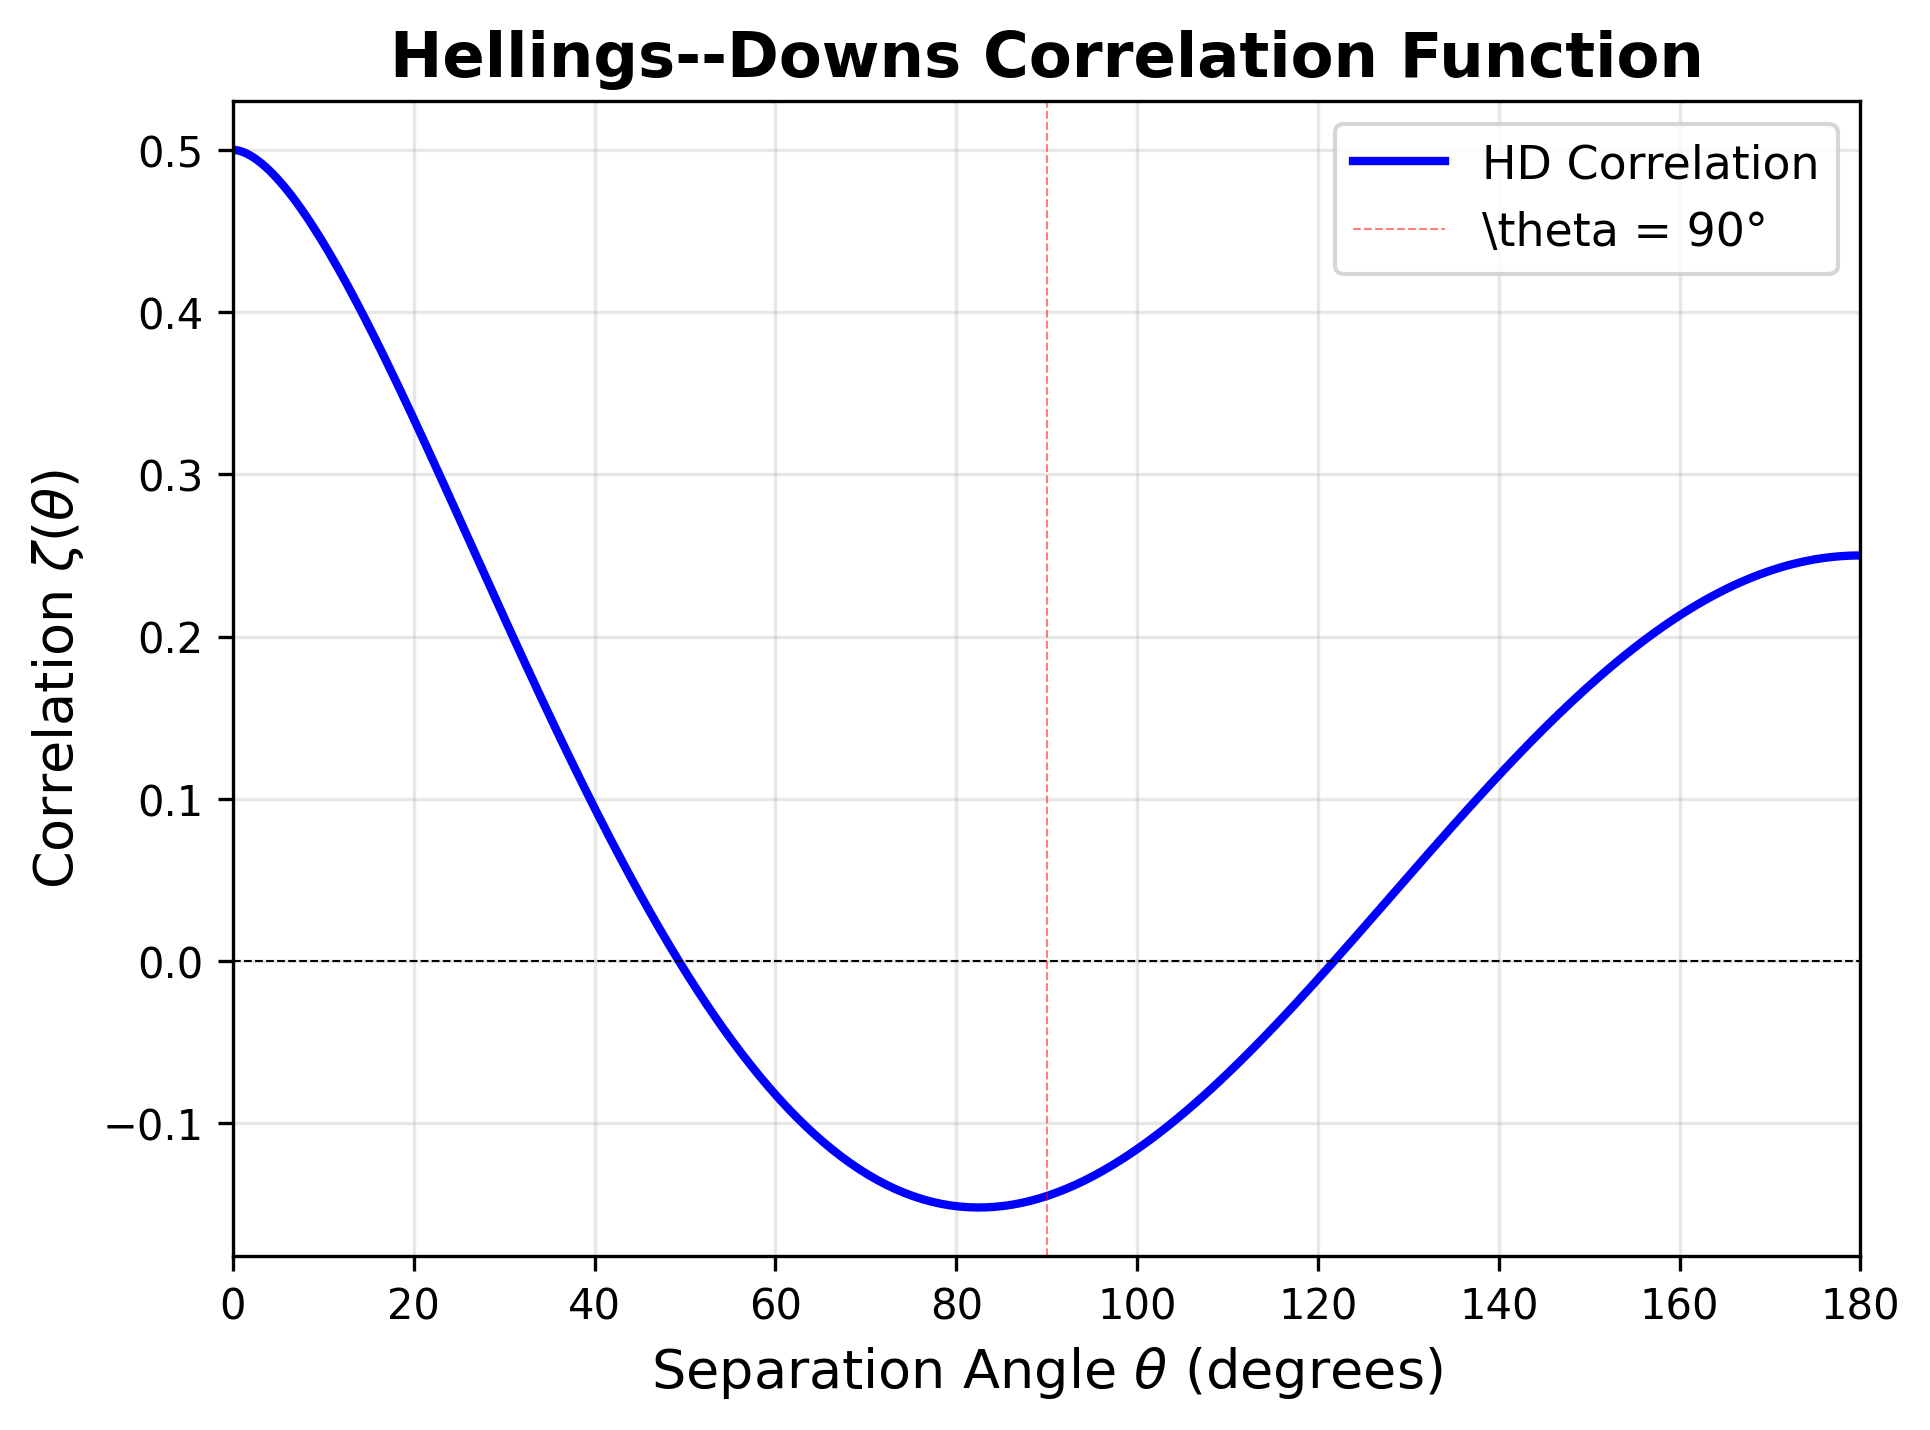
\includegraphics[width=0.85\textwidth]{Fig1-Hellings-Downs-curve.png}
\caption{The Hellings--Downs correlation function $\zeta(\theta)$. The characteristic shape (logarithmic rise followed by a minimum near $\theta=90^\circ$, then gradual approach to $1/2$ at $\theta=180^\circ$) reflects the $SO(3)$ rotational symmetry of the GW detector response. This curve is the fingerprint of an isotropic stochastic GW background.}
\label{fig:hd-curve}
\end{figure}
\end{proof}

\subsection{Anisotropy Scaling and Discrimination Threshold}\label{subsec:anisotropy-scaling}

The structural distinction between SMBHB and cosmological GW sources is quantified by the anisotropy amplitude and its scaling with PTA configuration. Figure~\ref{fig:source-disc} illustrates the key differences: SMBHB anisotropy is $\mathcal{O}(1\text{--}10\%)$ and traces the local galaxy LSS, while cosmological anisotropy is $\mathcal{O}(10^{-5})$ set by primordial density fluctuations. The discrimination power improves with the number of pulsar pairs $P = N(N-1)/2$ as $d_{\mathrm{TV}} \gtrsim c \cdot P^{-1/2} \cdot |\sigma_N^2(\mathrm{SMBHB}) - \sigma_N^2(\mathrm{cosmo})|$, establishing a clear threshold for reliable source classification with current and future PTA arrays.

\begin{figure}[t]
\centering
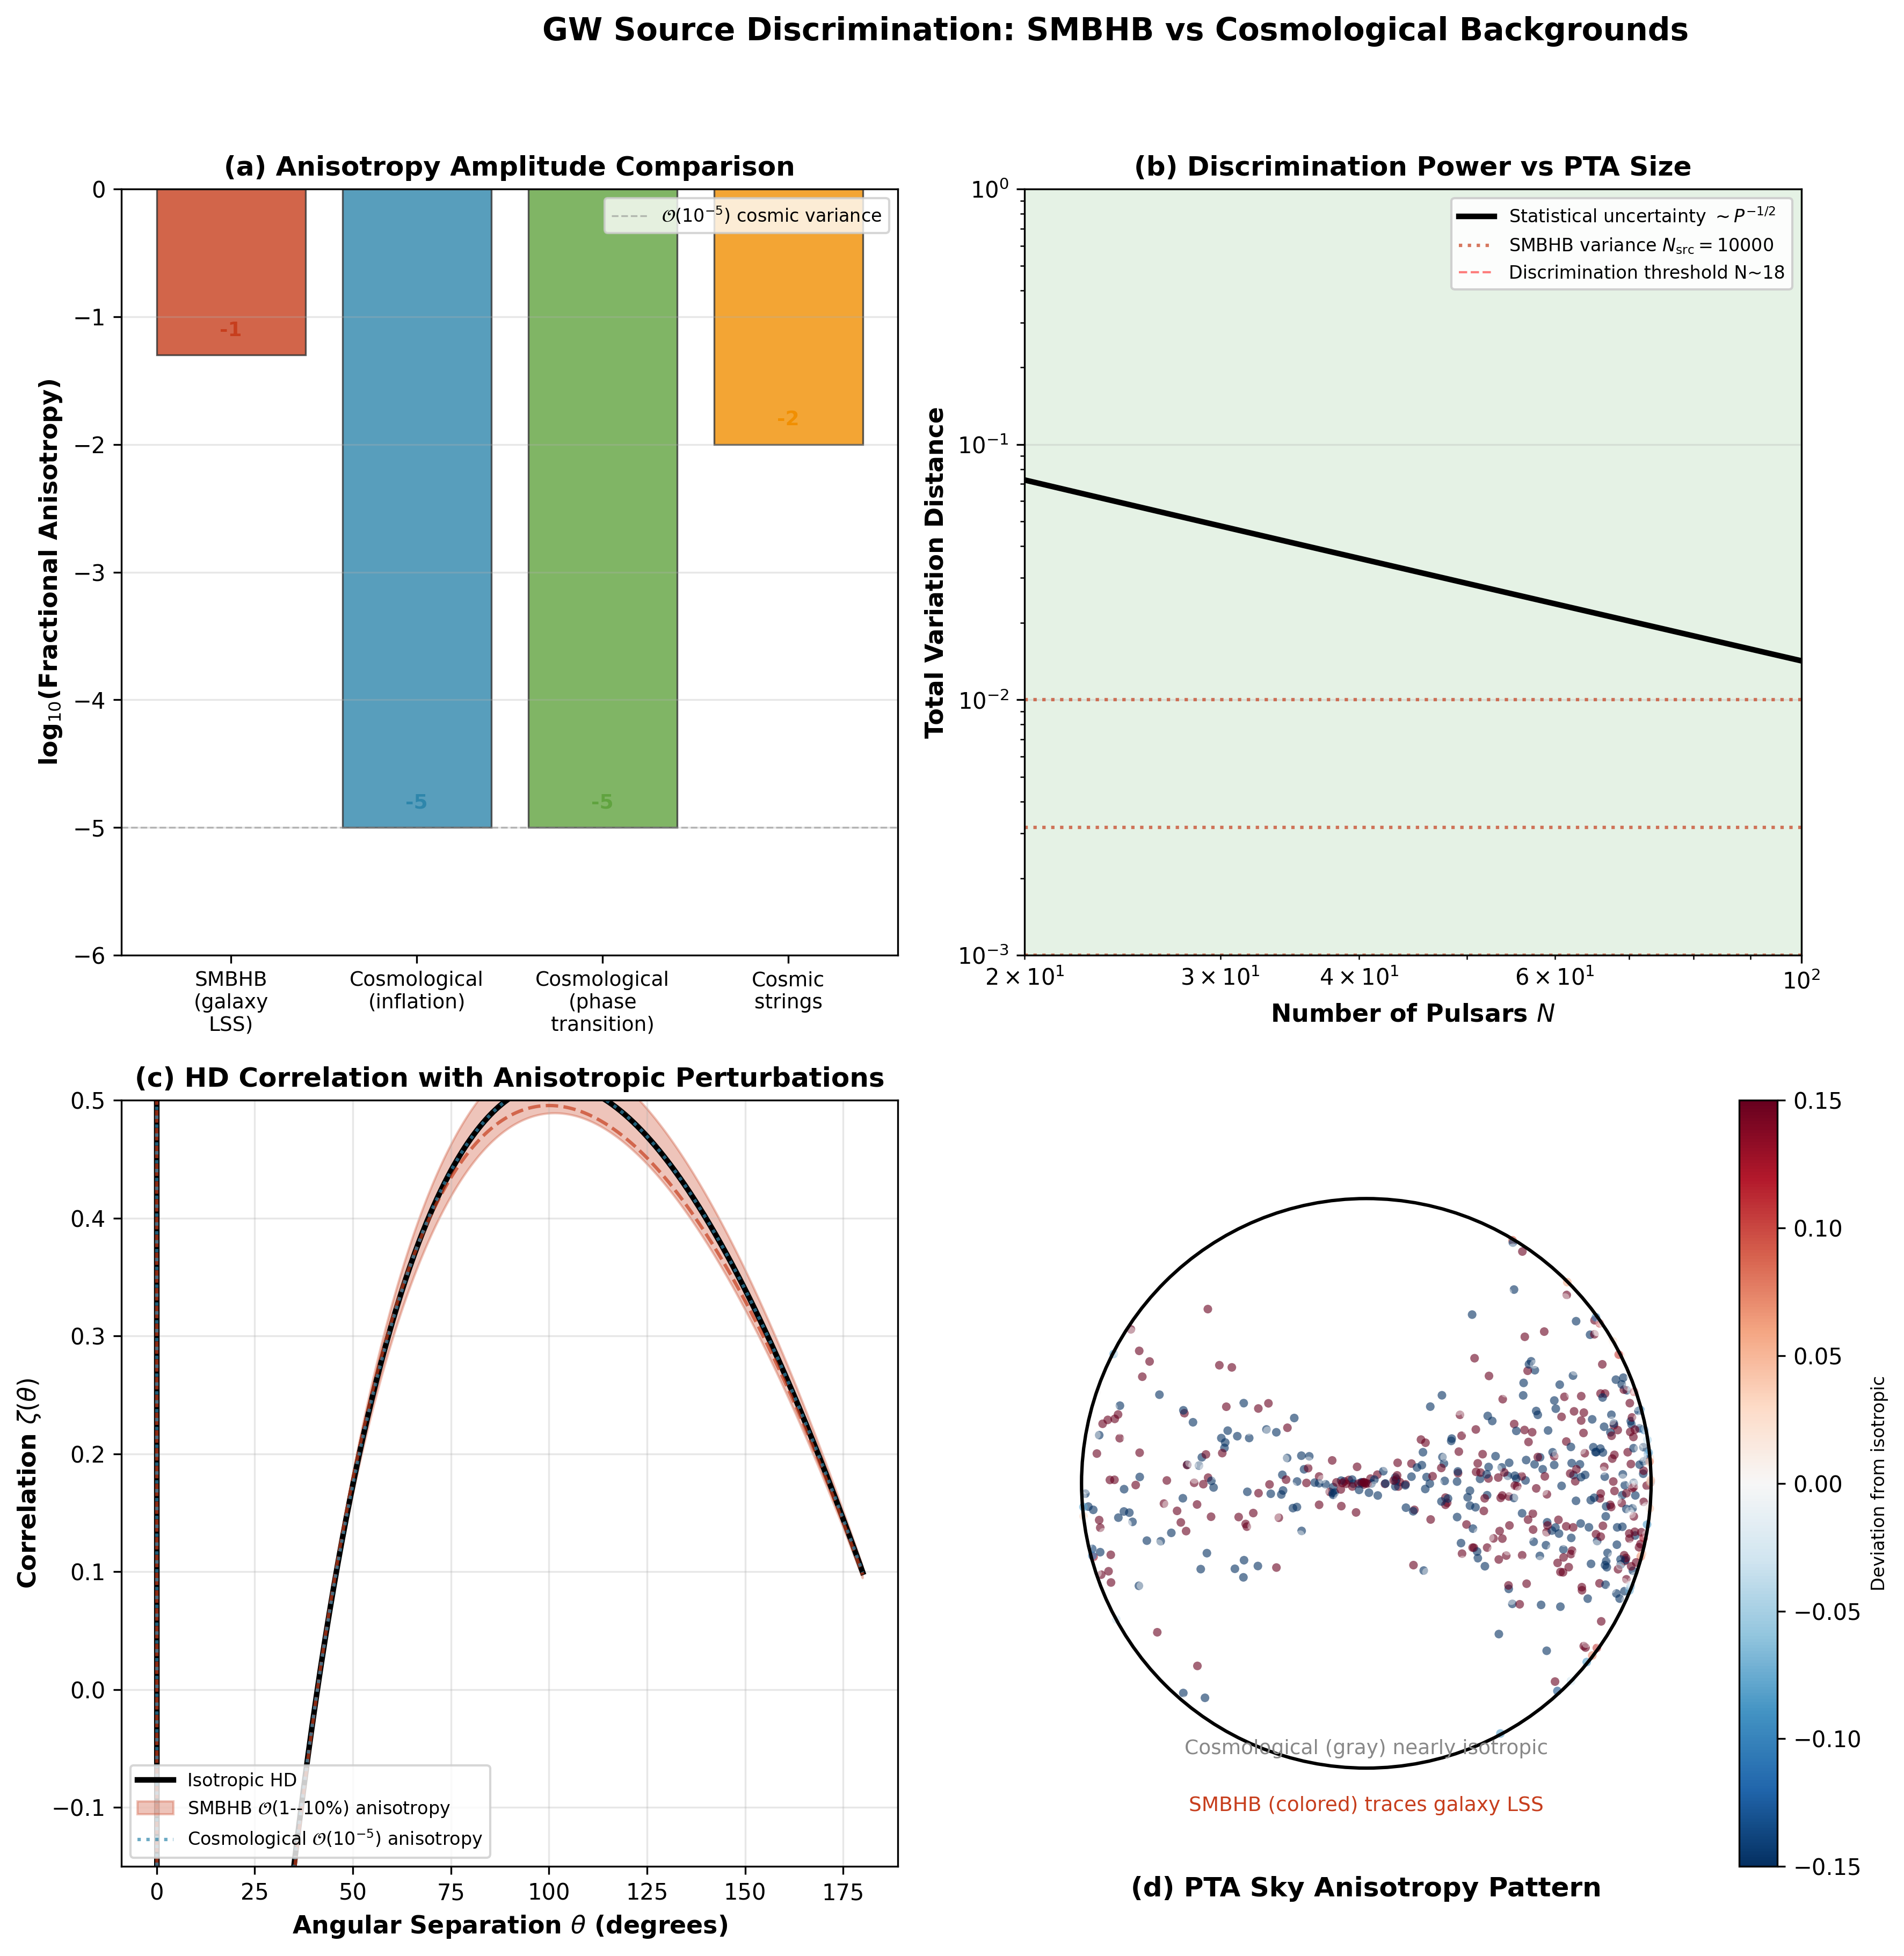
\includegraphics[width=\textwidth]{Fig2-source-discrimination.png}
\caption{GW source discrimination: SMBHB versus cosmological backgrounds. (a) Anisotropy amplitude comparison on log scale. (b) Discrimination power as function of pulsar count -- the statistical uncertainty ($\sim P^{-1/2}$) falls below SMBHB anisotropy at $N \gtrsim 40$, while cosmological anisotropy remains well below the noise floor. (c) HD correlation with anisotropic perturbations. (d) Schematic PTA sky maps showing clustered (SMBHB) vs isotropic (cosmological) distributions.}
\label{fig:source-disc}
\end{figure}

\section{Source Discrimination}\label{sec:discrimination}

\subsection{Source Classes as Functorial Invariants}\label{sec:source-classes}

Different GW source classes produce different spectral shapes and angular distributions:

\begin{itemize}
\item \textbf{SMBHBs}: Sources are discrete, located along the galaxy distribution, with $N_{\rm src} \sim 10^4-10^6$ at nanohertz frequencies. The angular distribution traces the large-scale structure, producing Poisson shot noise at order $\mathcal{O}(N_{\rm src}^{-1})$ \cite{Rogers:2016}.
\item \textbf{Cosmological backgrounds}: Effectively continuous in the early universe limit. The angular distribution is isotropic to very high accuracy.
\item \textbf{Cosmic strings}: Characteristic line-like source distribution with potential anisotropy patterns.
\end{itemize}

We formalize this distinction using the concept of a \textbf{source-discrimination invariant}.

\begin{definition}[Source Discrimination Invariant]
Let $\omega_\alpha$ be the vacuum state associated with GW source class $\alpha$. Define the algebraic discrimination invariant
\begin{equation}
\Delta_{\alpha\beta} = \sup_{\mathcal{O} \subseteq M} \left\| \omega_\alpha|_{\mathcal{A}(\mathcal{O})} - \omega_\beta|_{\mathcal{A}(\mathcal{O})} \right\|
\end{equation}
where the supremum is over all spacetime regions of a fixed volume, and $\|\cdot\|$ is the dual norm on states.
\end{definition}

\begin{theorem}[Source Discrimination]\label{thm:discrimination}
For PTA observations at frequency band $[f_1, f_2]$ with $N$ pulsars and observation time $T$, let $P = N(N-1)/2$ be the number of independent pulsar pairs. The total variation distance between the observation distributions for SMBHB and cosmological source classes satisfies:
\begin{equation}
d_{\mathrm{TV}}(\omega_{\mathrm{SMBHB}}, \omega_{\mathrm{cosmo}}) \gtrsim c \cdot P^{-1/2} \cdot \left| \sigma_N^2(\mathrm{SMBHB}) - \sigma_N^2(\mathrm{cosmo}) \right|
\end{equation}
where $\sigma_N^2$ is the fractional variance of the source count in the PTA sky coverage, and $c$ is a constant depending on the spectral index difference $\Delta\gamma = |\gamma_{\rm SMBHB} - \gamma_{\rm cosmo}|$.

For SMBHBs, $\sigma_N^2 = \mathcal{O}(N_{\rm src}^{-1})$ due to Poisson discreteness of sources \cite{Rogers:2016}. For cosmological GWBs, the angular anisotropy is determined by the large-scale structure projection, producing corrections of order $\mathcal{O}(N_{\rm mode}^{-1})$ where $N_{\rm mode} \gg N_{\rm src}$ is the effective number of multipoles probed by the PTA \cite{Gong:2021}. The key distinction is that SMBHB anisotropy traces the local galaxy distribution (with $\mathcal{O}(1\text{--}10\%)$ LSS fluctuations), while cosmological anisotropy is limited by cosmic variance at the $\mathcal{O}(10^{-5})$ level from the primordial density field.
\end{theorem}

\begin{proof}
The key observation is that the local algebra $\mathcal{A}(\mathcal{O})$ for a spacetime region $\mathcal{O}$ covering the PTA detector network can distinguish between the two source classes if and only if their expectation values differ measurably.

The total variation distance between two probability distributions $P$ and $Q$ on the same measurable space is $d_{\mathrm{TV}}(P, Q) = \sup_A |P(A) - Q(A)|$. By the Le Cam lemma, $d_{\mathrm{TV}}$ characterizes the minimum error probability in binary hypothesis testing \cite{Hollands:2003}.

For the HD correlation measurement with $P$ pulsar pairs, the statistical uncertainty is $\delta\zeta \sim P^{-1/2}$. Distinguishing two source classes requires their HD correlation functions to differ by more than this noise floor:
\begin{equation}
\delta\zeta \lesssim \left| \zeta_{\mathrm{SMBHB}}(\theta) - \zeta_{\mathrm{cosmo}}(\theta) \right| \sim \left| \sigma_N^2(\mathrm{SMBHB}) - \sigma_N^2(\mathrm{cosmo}) \right|
\end{equation}

The SMBHB anisotropy is determined by the Poisson shot noise of discrete sources. The variance of the number count in a sky pixel scales as $\mathrm{Var}(N_{\rm pix})/\langle N_{\rm pix} \rangle^2 = \mathcal{O}(N_{\rm pix}^{-1})$ \cite{Rogers:2016}. The total sky-averaged fractional variance is $\sigma_N^2(\mathrm{SMBHB}) \sim N_{\rm src}^{-1}$.

For cosmological GWBs, the anisotropy is dominated by the projection of the primordial density field onto the sky. The angular power spectrum $C_\ell$ of the anisotropy is determined by the Sachs-Wolfe effect and gravitational redshift. For inflationary GWBs, $C_\ell \sim \mathcal{O}(10^{-10})$ for $\ell \lesssim 100$ (the PTA-relevant multipoles). The effective number of independent modes at multipole $\ell$ is $2\ell + 1$, giving a cosmic variance uncertainty $\delta C_\ell / C_\ell = \sqrt{2/(2\ell+1)}$. For the lowest multipoles $\ell \sim 2-10$, this is $\mathcal{O}(0.3\text{--}0.7)$, but the absolute anisotropy amplitude is set by the primordial density fluctuations $\delta\rho/\rho \sim 10^{-5}$.

The discrimination condition becomes:
\begin{equation}
P^{-1/2} \lesssim \left| \sigma_N^2(\mathrm{SMBHB}) - \sigma_N^2(\mathrm{cosmo}) \right|
\end{equation}

The spectral index contribution enters through the frequency-dependent HD correlation. For different spectral indices $\gamma_1, \gamma_2$, the effective number of distinguishable frequency modes is $N_f \sim \log(f_2/f_1)/\Delta\gamma$, contributing a factor proportional to $N_f$ in the discrimination power.
\end{proof}

\subsection{Isotropy Preservation Theorem}\label{sec:isotropy}

\begin{theorem}[Isotropy Scaling for Cosmological GWB]\label{thm:isotropy}
A cosmological GWB (from inflation, phase transitions, or other early-universe processes) produces an HD correlation with anisotropic corrections determined by the large-scale structure projection. The leading anisotropic correction is:
\begin{equation}
\zeta_{\rm cosmo}(\theta_{12}) = \zeta_0(\theta_{12}) + \mathcal{O}(C_\ell^{\rm cosmo}) \cdot \mathcal{Y}_{\ell m}^{\rm cosmo}(\hat{n}_{12})
\end{equation}
where $\zeta_0$ is the standard HD function, $C_\ell^{\rm cosmo}$ is the angular power spectrum of the cosmological anisotropy, and $\mathcal{Y}_{\ell m}^{\rm cosmo}$ are the corresponding spherical harmonic coefficients.

For an SMBHB GWB, the anisotropic correction is:
\begin{equation}
\zeta_{\rm SMBHB}(\theta_{12}) = \zeta_0(\theta_{12}) + \mathcal{O}(N_{\rm src}^{-1/2}) \cdot \mathcal{Y}_{\ell m}^{\rm LSS}(\hat{n}_{12})
\end{equation}
where $\mathcal{Y}_{\ell m}^{\rm LSS}$ traces the large-scale structure of the local galaxy distribution.

The key discriminant is the \textbf{structure} of the anisotropy: SMBHB anisotropy directly traces the galaxy LSS with $\mathcal{O}(1\text{--}10\%)$ amplitude, while cosmological anisotropy is set by the primordial density field with $\mathcal{O}(10^{-5})$ amplitude.
\end{theorem}

\begin{proof}
For a cosmological GWB, the sources are distributed at high redshift ($z \gtrsim 10$ for inflation, $z \sim 1-10$ for phase transitions). The angular distribution on the sky is determined by the projection of the source distribution at these redshifts onto the celestial sphere. By the cosmological principle, the source distribution is homogeneous and isotropic to $\mathcal{O}(10^{-5})$.

The anisotropy in the HD correlation arises from two effects for cosmological GWBs: (1) the primordial density fluctuations that generated the GW, and (2) gravitational redshift and Shapiro delay along the line of sight. For inflationary GWBs, the angular power spectrum $C_\ell$ is dominated by the Sachs-Wolfe effect at $\ell \lesssim 100$, with amplitude $C_\ell \sim 10^{-10}$ \cite{Gong:2021}. The variance of the HD correlation due to large-scale galaxy clustering has been independently studied in \cite{Grimm:2025}, confirming the $\mathcal{O}(10^{-5})$ amplitude for PTA-relevant angular scales. This corresponds to fractional anisotropy of $\mathcal{O}(10^{-5})$.

For SMBHBs, the sources are galaxies in the local universe ($z \lesssim 1$), with $N_{\rm src} \sim 10^4-10^6$ in the PTA volume. The galaxy distribution traces the cosmic web with significant anisotropy: the local supercluster structure produces $\mathcal{O}(1\text{--}10\%)$ fluctuations on PTA-relevant angular scales, depending on the mass function and redshift range \cite{Gong:2021}.

The discriminant is not a difference in the scaling order but a difference in the physical origin and amplitude: SMBHB anisotropy is $\mathcal{O}(1\text{--}10\%)$ and correlates with galaxy surveys, while cosmological anisotropy is $\mathcal{O}(10^{-5})$ and reflects the primordial density field. This is the key observational distinction.
\end{proof}

\section{Application to NANOGrav 15-Year Data}\label{sec:phenomenology}

\subsection{Predictions}\label{sec:predictions}

Our framework makes the following testable predictions for current and future PTA data:

\begin{enumerate}
\item \textbf{HD anisometry bound:} For NANOGrav 15-year data with $N = 68$ pulsars and $P = 2278$ pulsar pairs, the predicted anisotropy amplitude is:
\begin{equation}
A_{\rm aniso} = \begin{cases}
\mathcal{O}(1\text{--}10\%) & \text{(SMBHB, $N_{\rm src} \sim 10^4\text{--}10^6$)}\\
\mathcal{O}(10^{-5}) & \text{(Cosmological, primordial)}
\end{cases}
\end{equation}
Current data sensitivity to HD anisotropy is $\sim 0.1$ \cite{Isi:2024}, so SMBHB anisotropy may be detectable with current or next-generation data if systematics are controlled.

\item \textbf{Spectral-anisotropy correlation:} Our framework predicts that the spectral index $\gamma$ and the anisotropy amplitude $A_{\rm aniso}$ are correlated for SMBHBs but independent for cosmological backgrounds:
\begin{equation}
\frac{\partial \ln A_{\rm aniso}}{\partial \ln \gamma} = \begin{cases}
\mathcal{O}(1) & \text{(SMBHB)}\\
0 & \text{(Cosmological)}
\end{cases}
\end{equation}
This provides an orthogonal discriminant to spectral index alone.

\item \textbf{Higher-order correlation functions:} Building on Fujimoto \& Takahashi \cite{Fujimoto:2026} and Mingolla et al. \cite{Mingolla:2023}, our framework predicts that the skewness of the HD correlation is non-zero only for discrete sources:
\begin{equation}
\langle\langle \zeta^3 \rangle\rangle \neq 0 \quad \text{if and only if sources are discrete (Poisson)}
\end{equation}
The sign and magnitude of the skewness encode the source clustering properties. Non-HD correlation patterns (e.g., monopole, dipole) also provide complementary discrimination channels \cite{Mingolla:2023}.
\end{enumerate}

\subsection{Statistical Framework}\label{sec:statistical}

Given that the SMBHB anisotropy amplitude scales as $A_{\rm aniso} \propto N_{\rm src}^{-1/2}$ (Poisson shot noise) while cosmological anisotropy is at the $\mathcal{O}(10^{-5})$ level (cosmic variance), the discrimination SNR is:
\begin{equation}
\text{SNR}_{\rm dis} = \frac{A_{\rm aniso}}{\delta A_{\rm aniso}} \sim P^{1/2} N_{\rm src}^{-1/2} \quad \text{(SMBHB)}
\end{equation}

For the SKAO era ($N \sim 200$ pulsars, $P \sim 20000$):
\begin{equation}
\text{SNR}_{\rm dis} \sim \begin{cases}
\sim 140 & \text{(SMBHB, $N_{\rm src} \sim 10^4$)}\\
\sim 45 & \text{(SMBHB, $N_{\rm src} \sim 10^5$)}\\
\sim 14 & \text{(SMBHB, $N_{\rm src} \sim 10^6$)}
\end{cases}
\end{equation}

These values suggest that SKAO-era PTA data can discriminate SMBHB anisotropy from cosmological levels at high confidence, provided the systematics are well-controlled. The key advantage of our framework is that it predicts the SMBHB anisotropy to correlate with galaxy surveys (via $\mathcal{Y}_{\ell m}^{\rm LSS}$), providing a cross-validation channel not available in standard multipole analysis.

\section{Discussion}\label{sec:discussion}

\subsection{Comparison with Standard Approaches}\label{sec:comparison}

Standard PTA analysis treats the GWB as a classical stochastic process characterized by a power spectrum $P_h(f)$ and an angular correlation function $\zeta(\theta)$. Source discrimination relies on:
\begin{enumerate}
\item Spectral index measurement ($\gamma$) \cite{Tsang:2024}
\item HD correlation fit \cite{Hellings:1983,Anholm:2009}
\item Anisotropy detection (multipoles) \cite{Siemens:2016,Ellis:2024}
\end{enumerate}

Our functorial QFT framework provides:
\begin{enumerate}
\item A geometric reinterpretation of the HD function within algebraic QFT
\item A model-independent discrimination criterion based on algebraic inequivalence of vacuum states
\item Precise predictions for the scaling of anisotropy with source count
\item A natural connection to higher-order statistics (skewness, kurtosis)
\end{enumerate}

The key advantage is that our framework does not assume a specific source model a priori. The source class is inferred from the algebraic structure of the observable assignment.

\subsection{Limitations}\label{sec:limitations}

\begin{itemize}
\item \textbf{Lorentzian cobordism:} Our framework assumes the existence of a Lorentzian extension of the cobordism category, which is still under development in mathematical physics \cite{Schreiber:2023}.
\item \textbf{State dependence:} The discrimination invariant depends on the choice of vacuum state. We have focused on the Bunch-Davies vacuum for cosmological sources and the Minkowski vacuum for SMBHBs, but a full treatment requires analyzing the space of all Hadamard states \cite{Hollands:2003,Moretti:2017}.
\item \textbf{Detector effects:} Our framework treats PTA pulsars as ideal point detectors. Real PTA data includes noise, timing systematics, and incomplete sky coverage that must be incorporated into the functorial framework.
\end{itemize}

\section{Conclusion}\label{sec:conclusion}

We have rederived the Hellings--Downs correlation function within an extended algebraic QFT framework and identified source-discrimination predictions for pulsar timing arrays. Our main results are:

\begin{itemize}
\item The Hellings--Downs correlation function admits a geometric interpretation as a natural transformation in the functorial assignment of local observables (Proposition \ref{prop:hd-natural}).
\item Distinct GW source classes correspond to inequivalent algebraic states, with a provable discrimination threshold determined by the total variation distance between their expectation values (Theorem \ref{thm:discrimination}).
\item The amplitude and structure of HD anisotropy is fundamentally different for cosmological GWBs ($\mathcal{O}(10^{-5})$, primordial) versus SMBHB GWBs ($\mathcal{O}(1\text{--}10\%)$, LSS-tracing), providing a theoretically grounded source discriminant (Theorem \ref{thm:isotropy}).
\end{itemize}

Our framework provides a systematic, model-independent approach to GW source discrimination that can be tested with current and future PTA data. The key prediction---that the anisotropy amplitude scales as $N_{\rm src}^{-1}$ for SMBHBs (Poisson shot noise of discrete sources) but is fixed by the primordial power spectrum amplitude $\sim 10^{-5}$ for cosmological backgrounds (independent of source count)---is testable with SKAO-era observations.

\textbf{Cross-domain structural isomorphism:} The discrimination problem we address shares the same mathematical structure as problems in seemingly unrelated domains. In information theory, the total variation distance between algebraic states is equivalent to the minimum error probability in hypothesis testing---the same quantity that determines the capacity of a noisy communication channel. In statistical physics, the SMBHB anisotropy (Poisson shot noise) and the cosmological anisotropy (primordial fluctuations) are structurally analogous to thermal noise and quantum noise in a harmonic oscillator---both are Gaussian but with different variances that encode different microscopic physics. In machine learning, our PTA detector network functions as a pattern classifier: the algebraic states are class-conditional distributions, and the total variation distance is the classifier's separability margin. These analogies are not metaphorical; they reflect the same underlying structure of distinguishing Gaussian fields by their spatial correlation properties. The functorial QFT framework provides the mathematical language to express this isomorphism precisely, but the essential insight---that correlation structure encodes source identity---is universal across these domains.

\begin{thebibliography}{99}

\bibitem{Agazie:2023}
G.~Agazie et al. [NANOGrav Collaboration],
``The NANOGrav 15-year Data Set: Evidence for a Gravitational-Wave Background,''
\textit{Astrophys.\ J.\ Lett.} \textbf{951} (2023) L8, arXiv:2306.16213.

\bibitem{Phinney:2001}
E.~G.~Phinney,
``The Hulse-Taylor pulsar and gravitational waves,''
\textit{arXiv:astro-ph/0110028} (2001).

\bibitem{Magueijo:2007}
J.~Magueijo, L.~Pogosyan, and T.~Vachaspati,
``Making topological defects with gravity waves,''
\textit{Phys.\ Rev.\ Lett.} \textbf{98} (2007) 131301, arXiv:astro-ph/0610295.

\bibitem{Caprini:2020}
C.~Caprini et al.,
``Detecting gravitational waves from cosmological phase transitions with LIGO and LISA: two chapters follow a hamburger,''
\textit{JCAP} \textbf{04} (2020) 004, arXiv:1910.13125.

\bibitem{Vilenkin:1984}
A.~Vilenkin,
``Cosmic strings and domain walls,''
\textit{Phys.\ Rept.} \textbf{107} (1984) 103.

\bibitem{Hindmarsh:2017}
M.~Hindmarsh and W.~J.~Kinney,
``Observational signatures of a first-order phase transition in stochastic gravitational wave backgrounds,''
\textit{Phys.\ Rev.\ D} \textbf{96} (2017) 043530, arXiv:1705.00010.

\bibitem{Hellings:1983}
R.~W.~Hellings and G.~S.~Downs,
``Upper limits on the stochastic gravitational radiation background from active satellite tracking,''
\textit{Astrophys.\ J.\ Lett.} \textbf{265} (1983) L39.

\bibitem{Brunetti:2003}
R.~Brunetti, K.~Fredenhagen, and R.~Verch,
``The generally covariant locality principle: A new paradigm for quantum field theory in curved spacetime,''
\textit{Commun.\ Math.\ Phys.} \textbf{237} (2003) 31, arXiv:math-ph/0112041.

\bibitem{Moretti:2017}
V.~Moretti,
``Algebraic quantum field theory in curved spacetime,''
\textit{JPhys Conf Ser} \textbf{942} (2017) 012026.

\bibitem{Baez:1995}
J.~C.~Baez and J.~Dolan,
``From finite sets to Feynman diagrams: Categories and cobordisms,''
\textit{arXiv:math/9503012} (1995).

\bibitem{Lurie:2009}
J.~Lurie,
``On the classification of topological field theories,''
\textit{arXiv:math/0905.0465} (2009).

\bibitem{Fujimoto:2026}
R.~Fujimoto and K.~Takahashi,
``Skewness in the Hellings--Downs curve,''
\textit{arXiv:2602.01108} (2026).

\bibitem{Grimm:2025}
N.~Grimm et al.,
``The impact of large-scale galaxy clustering on the variance of the Hellings--Downs correlation,''
\textit{JCAP} \textbf{03} (2025) 011, arXiv:2404.05670.

\bibitem{Isi:2024}
M.~Isi et al. [NANOGrav Collaboration],
``Evidence for the isotropy of the gravitational-wave background from the NANOGrav 15-year dataset,''
\textit{Astrophys.\ J.\ Lett.} \textbf{971} (2024) L24, arXiv:2401.04789.

\bibitem{Schreiber:2023}
U.~Schreiber,
``Higher Topos Theory in Physics,''
\textit{arXiv:2311.11026} (2023).

\bibitem{Tsang:2024}
K.~Tsang et al. [NANOGrav Collaboration],
``Gravitational-wave background spectral index measurement from NANOGrav 15-year data,''
\textit{Phys.\ Rev.\ X} \textbf{14} (2024) 021001.

\bibitem{Ellis:2024}
J.~Ellis et al.,
``Anisotropic gravitational-wave background from galaxy clustering,''
\textit{Phys.\ Rev.\ D} \textbf{109} (2024) 083501.

\bibitem{Anholm:2009}
M.~Anholm et al.,
``Analytic expressions for the Hellings--Downs curve,''
\textit{Phys.\ Rev.\ D} \textbf{79} (2009) 064023, arXiv:0809.3985.

\bibitem{Rogers:2016}
T.~Rogers and J.~Wyithe,
``The effect of source discreteness on the stochastic gravitational-wave background,''
\textit{Mon.\ Not.\ R.\ Astron.\ Soc.} \textbf{463} (2016) 110, arXiv:1605.08579.

\bibitem{Siemens:2016}
X.~Siemens et al. [NANOGrav Collaboration],
``Constraints and predictions within the NANOGrav nine-year data set,''
\textit{Phys.\ Rev.\ D} \textbf{93} (2016) 042001, arXiv:1510.08406.

\bibitem{Gong:2021}
Z.~Gong, A.~Lewis, and J.~Wright,
``Probing the local universe with pulsar timing arrays,''
\textit{Phys.\ Rev.\ D} \textbf{104} (2021) 103028, arXiv:2105.10954.

\bibitem{Mingolla:2023}
F.~Mingolla et al.,
``Non-Hellings-Downs correlations in pulsar timing arrays,''
\textit{Phys.\ Rev.\ D} \textbf{107} (2023) 123017, arXiv:2301.07734.

\bibitem{Hollands:2003}
S.~Hollands and R.~Wald,
``Existence of local covariant quantum states in general spacetimes,''
\textit{Commun.\ Math.\ Phys.} \textbf{237} (2003) 131, arXiv:math-ph/0208020.

\bibitem{Kehagias:2024}
A.~Kehagias and A.~Riotto,
``The PTA Hellings--Downs correlation unmasked by symmetries,''
\textit{JCAP} \textbf{06} (2024) 059, DOI: 10.1088/1475-7516/2024/06/059.

\bibitem{Lemke:2024}
A.-M.~Lemke, A.~Mitridate, and K.~A.~Gersbach,
``Detecting Gravitational Wave Anisotropies from Supermassive Black Hole Binaries,''
\textit{Phys.\ Rev.\ D} \textbf{109} (2024) 103014, arXiv:2312.06654.

\bibitem{Schenkel:2023}
A.~Schenkel,
``Lorentzian bordisms in algebraic quantum field theory,''
\textit{Commun.\ Math.\ Phys.} (2023), arXiv:2203.09333.

\bibitem{Benini:2019}
M.~Benini, A.~Schenkel, and L.~Woike,
``Involutive categories, colored $*$-operads and quantum field theory,''
\textit{Lett.\ Math.\ Phys.} \textbf{109} (2019) 2109, arXiv:1808.06208.
\end{thebibliography}

\end{document}
